\chapter{Systematic uncertainties on simulated samples}\label{chap:sysmc}

There are several systematics that effect the background modelling of the simulated samples, these uncertainties can be divided into two distinct categories: experimental uncertainties related to the event (e.g luminosity measurement) and reconstruction of the physics objects described in \cref{chap:SimReco}, and uncertainties of theoretical predictions from the PDF and the choice of PDF. Due to the data-driven nature of the analysis, uncertainties related to the simulated samples background modelling are not directly applied, instead, they are propagated to calculating the bias introduced on the background model choice. Further detail on the background model uncertainties are given in \cref{chap:bkgmodel}. The theoretical background uncertainty variations are estimated as a function of $m_{ll}$ at truth mass and the transfer function approach, described in \cref{sec:datamc:transfer}, is applied to generate smooth reconstructed templates for the uncertainties. Furthermore, uncertainties on the fake-template estimation is also considered to estimate the impact on the background model. The experimental uncertainties are provided by dedicated groups in charge of performance of electron and muon reconstruction and measurement.

\section{Experimental uncertainties}\label{sec:sysmc:exp}

\subsection{Event Uncertainties}
Uncertainty on the luminosity and the pileup measurements affect the overall normalisaton of the processes being studied. The determination of the luminosity is described in \cref{sec:method:lumi} and the uncertainty is calculated using the method described in \cite{Aaboud:2208146}. For the full Run-2 dataset used in this analysis the luminosity uncertainty was found to be $\pm 1.7\%$. The uncertainty on the pileup distributions by taking the difference between the pileup distribution observed in data and those expected at the time of producing the MC simulations. Additionally, uncertainties on the efficiency of the triggers used in the analysis is also considered.  \cref{fig:uncert:prwuncert} depicts the effect of the pileup uncertainty on the invariant mass distribution for the electron and muon channels. A difference between the electron and muon channels can be seen for the pileup uncertainty due to statistical fluctuations in the simulated sample. 
\begin{figure}[h!]
    \centering
    \begin{subfigure}[h]{0.42\textwidth}
        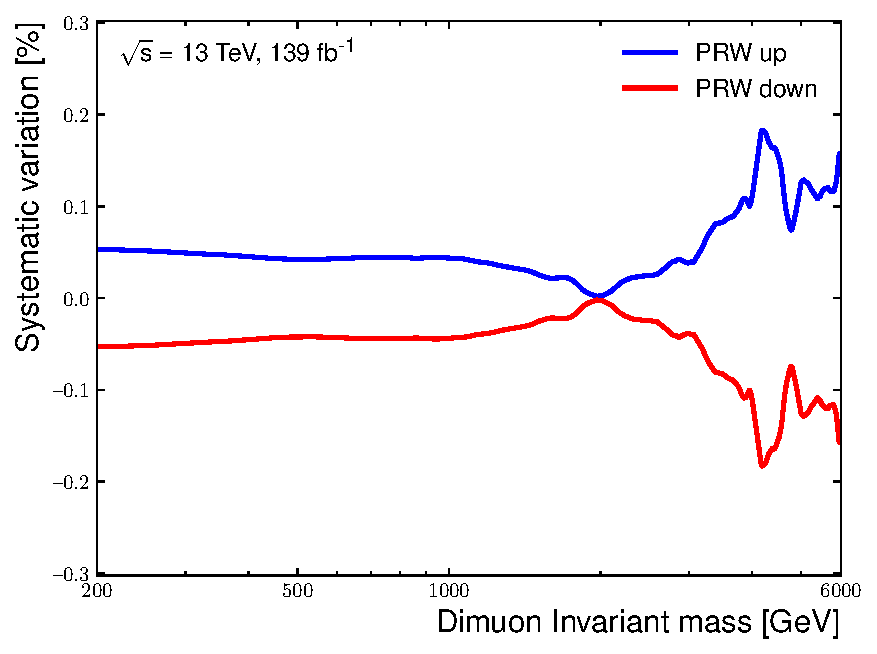
\includegraphics[width=\textwidth]{figures/analysis/datamc/Uncertainties/exp/mm/m_uu_pstOR_PRW_DATASF__1up.pdf}
        \label{fig:uncert:mmprw}
    \end{subfigure}
    \begin{subfigure}[h]{0.42\textwidth}
        \centering
        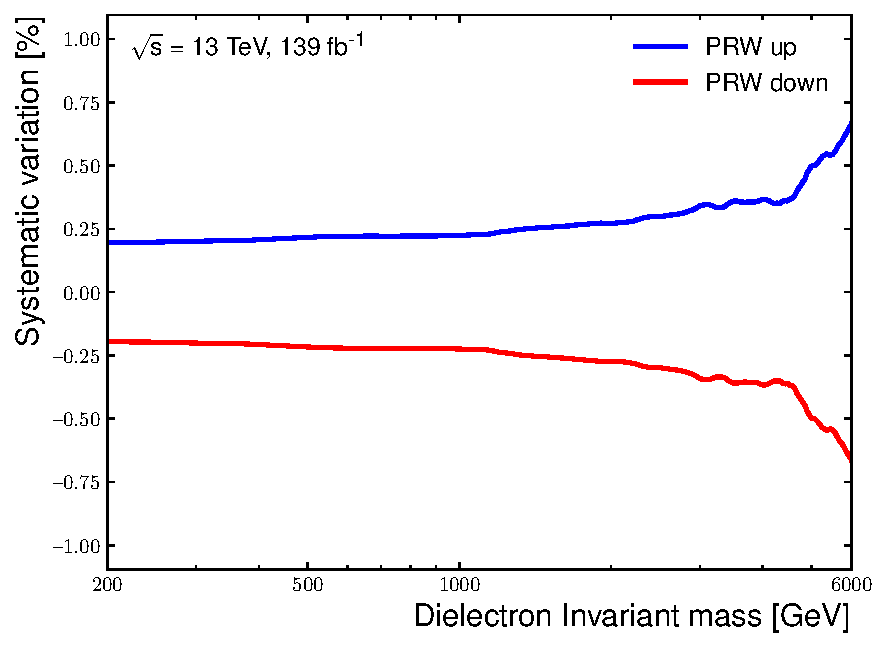
\includegraphics[width=\textwidth]{figures/analysis/datamc/Uncertainties/exp/ee/m_ee_pstOR_PRW_DATASF__1up.pdf}
        \label{fig:uncert:eeprw}
    \end{subfigure}
    \caption[Systematic uncertainty due to pileup reweighting]{Systematic uncertainties due to pileup in the muon (left) and electron (right).}
    \label{fig:uncert:prwuncert}
\end{figure}

\subsection{Lepton uncertainties}

\subsubsection{Efficiencies}
The electron and muon efficiency uncertainties are obtained by using the tag-and-probe method~\cite{Aaboud:2016vfy,Aad:2016jkr} by varying the selection of identification, isolation and trigger criteria individually~\cite{Aad:2019tso,Aad:2016jkr}. Therefore, providing efficiency uncertainties for the isolation, identification and trigger criteria. The efficiency is only calculated up to the \et of \SI{150}{\giga\electronvolt}, as a result, an extrapolation procedure is performed to provide an estimate of the uncertainty at higher \et. Further detail on the efficiency uncertainty calculations are provided in \cite{Aad:2019tso,Aad:2016jkr} for electrons and muons, respectively. 

\subsubsection{Resolution}
Smearing of the electron energies in MC accounts for the differences in energy resolution between data and MC. A full correlation model for energy resolution uncertainty consists of several nuisance parameters where all uncertainties have been decorrelated in bins of $\eta$~\cite{Aad:2019tso}.

The muon resolution corrections are calculated by fitting several correction coefficients that is used to match the invariant mass distributions between MC and data. Each fit parameter in the model is associated with a source of potential disagreement between data and MC. The uncertainty on the resolution is derived by taking the variations of the fit procedure, the background parameterisation and muon spectrometer alignment~\cite{Aad:2016jkr}. 

\subsubsection{Energy scale}
Electron and muon energy scale corrections are applied only on data. The effects of varying the respective uncertainties associated with the energy scale corrections up and down is calculated to determine the systematic uncertainty and is calculated on MC due to the higher statistics available~\cite{Aad:2019tso}. 

\cref{fig:uncert:eeExp,fig:uncert:mmExp} depicts effects of uncertainties due to experimental sources on the invariant mass distributions for the electron and muon channels. 

\begin{figure}[]
    \centering
    \begin{subfigure}[b]{0.42\textwidth}
        \centering
        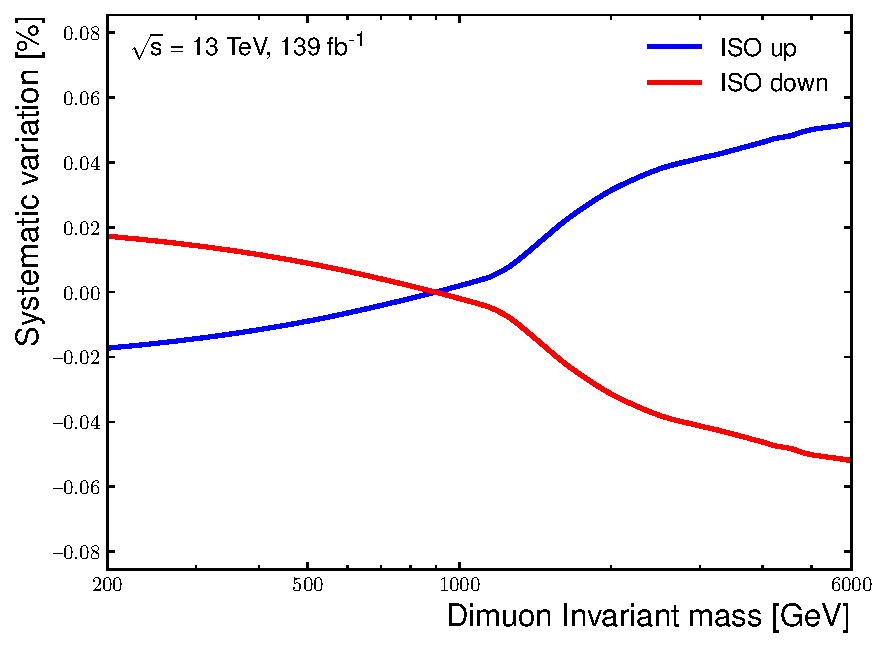
\includegraphics[width=\textwidth]{figures/analysis/datamc/Uncertainties/exp/mm/m_uu_pstOR_MUON_EFF_ISO_SYS__1up.pdf}
        \label{fig:uncert:mmIso}
    \end{subfigure}
    \begin{subfigure}[b]{0.42\textwidth}
        \centering
        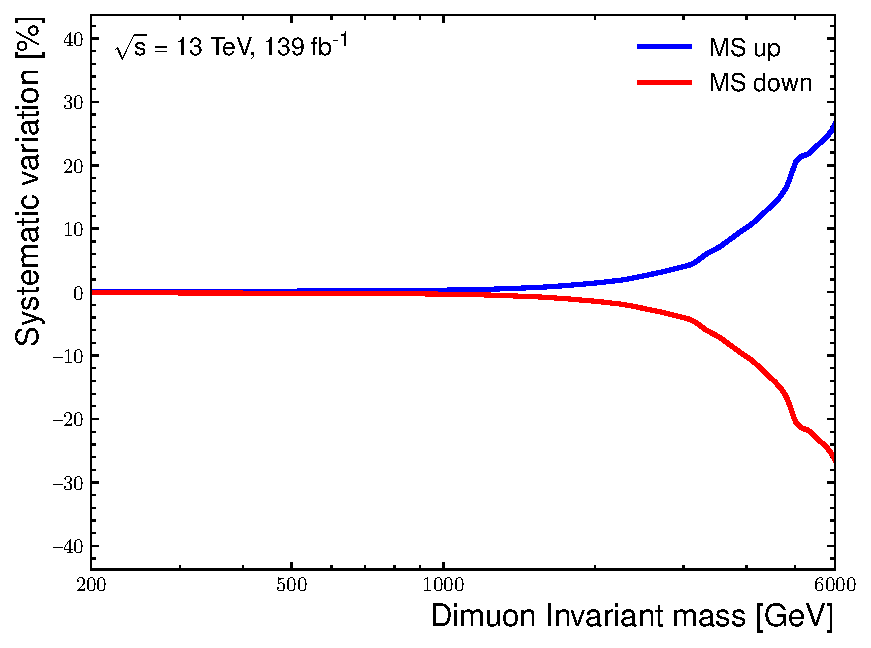
\includegraphics[width=\textwidth]{figures/analysis/datamc/Uncertainties/exp/mm/m_uu_pstOR_MUON_MS__1up.pdf}
        \label{fig:uncert:mmMC}
    \end{subfigure}
    \begin{subfigure}[b]{0.42\textwidth}
        \centering
        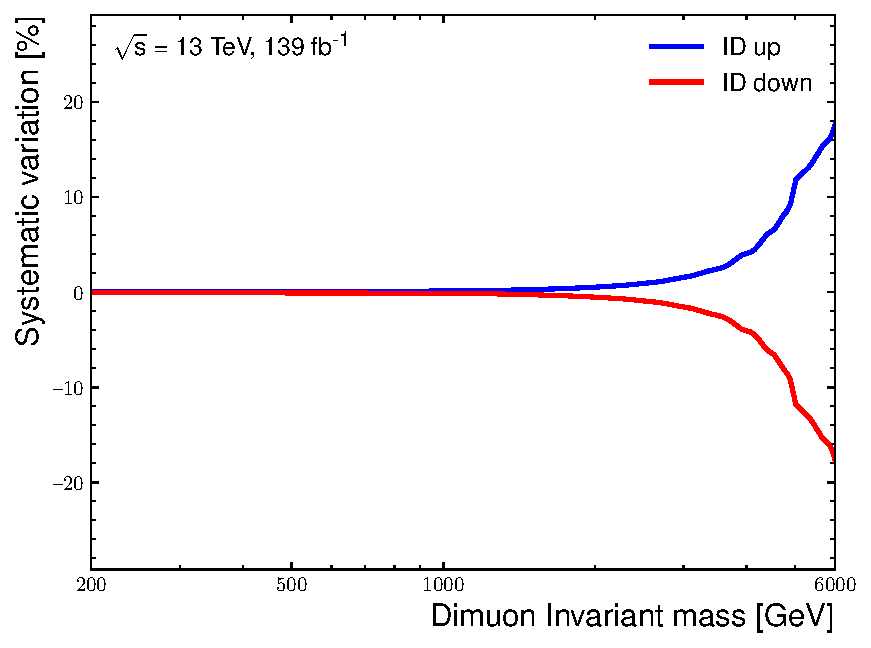
\includegraphics[width=\textwidth]{figures/analysis/datamc/Uncertainties/exp/mm/m_uu_pstOR_MUON_ID__1up.pdf}
        \label{fig:uncert:mmID}
    \end{subfigure}
    \begin{subfigure}[b]{0.42\textwidth}
        \centering
        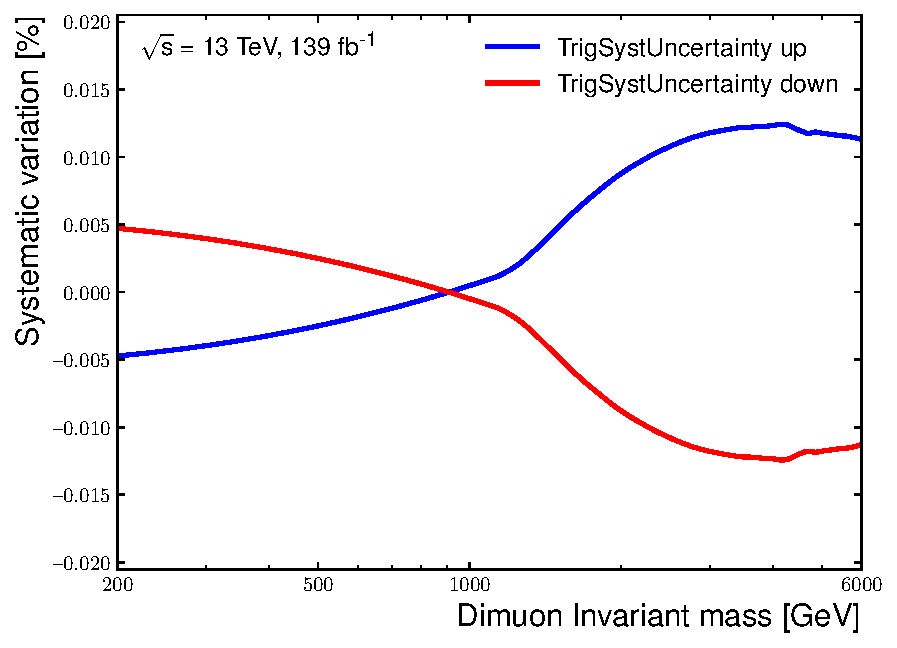
\includegraphics[width=\textwidth]{figures/analysis/datamc/Uncertainties/exp/mm/m_uu_pstOR_MUON_EFF_TrigSystUncertainty__1up.pdf}
        \label{fig:uncert:mmTrig}
    \end{subfigure}
    \begin{subfigure}[b]{0.42\textwidth}
        \centering
        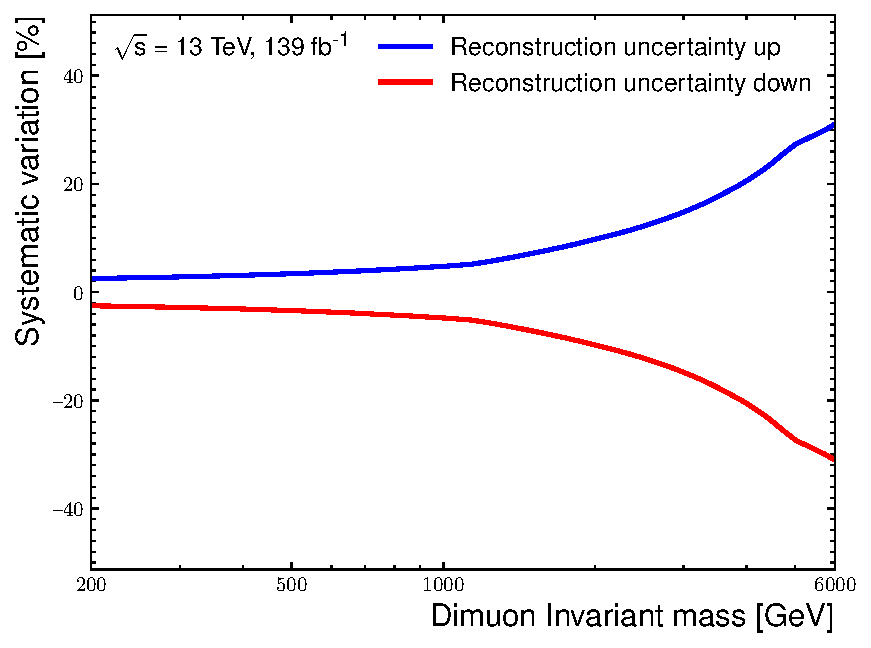
\includegraphics[width=\textwidth]{figures/analysis/datamc/Uncertainties/exp/mm/m_uu_pstOR_MUON_EFF_RECO_SYS__1up.pdf}
        \label{fig:uncert:mmReco}
    \end{subfigure}
    \begin{subfigure}[b]{0.42\textwidth}
        \centering
        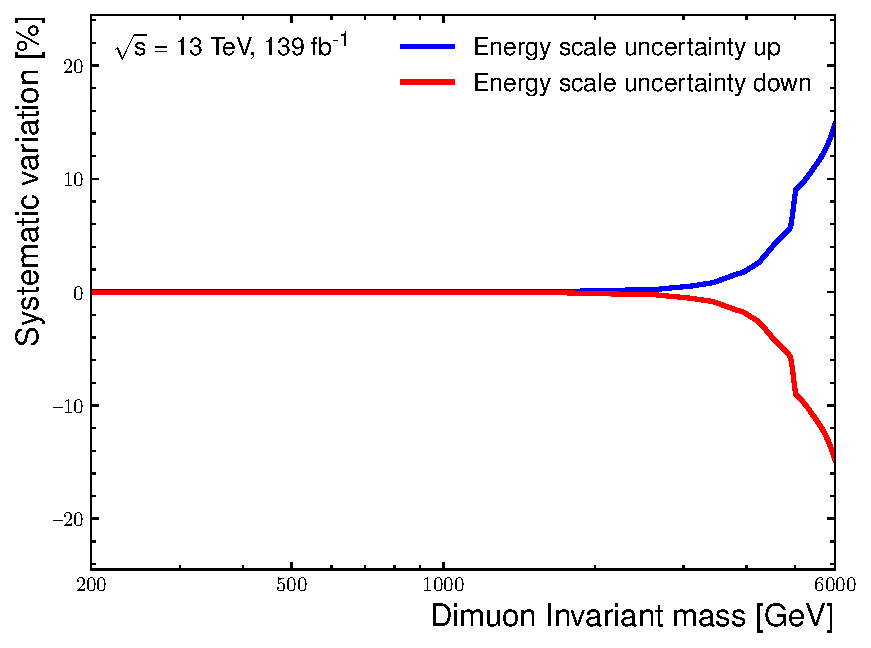
\includegraphics[width=\textwidth]{figures/analysis/datamc/Uncertainties/exp/mm/m_uu_pstOR_MUON_SCALE__1up.pdf}
        \label{fig:uncert:mmScale}
    \end{subfigure}
    \caption[Muon systematic uncertainties due to experimental sources]{Muon systematic uncertainties due to experimental sources. Shown from left to right and top to bottom, the uncertainty related to Isolation, momentum resolution in the MS and ID, identification, Trigger, reconstruction, and muon energy scale.}
    \label{fig:uncert:mmExp}
\end{figure}

\begin{figure}[]
    \centering
    \begin{subfigure}[b]{0.42\textwidth}
        \centering
        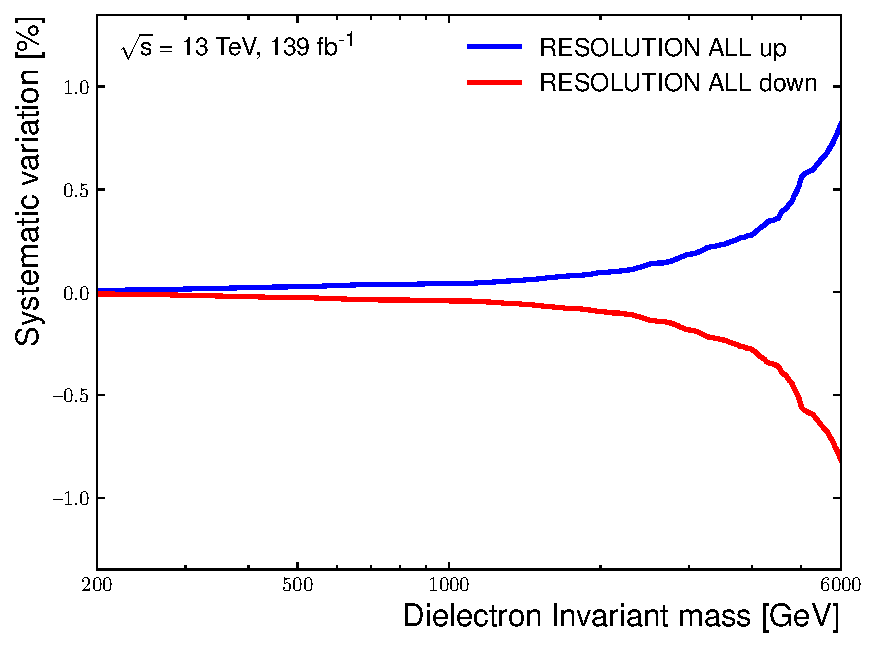
\includegraphics[width=\textwidth]{figures/analysis/datamc/Uncertainties/exp/ee/m_ee_pstOR_EG_RESOLUTION_ALL__1up.pdf}
        \label{fig:uncert:eeRes}
    \end{subfigure}
    \begin{subfigure}[b]{0.42\textwidth}
        \centering
        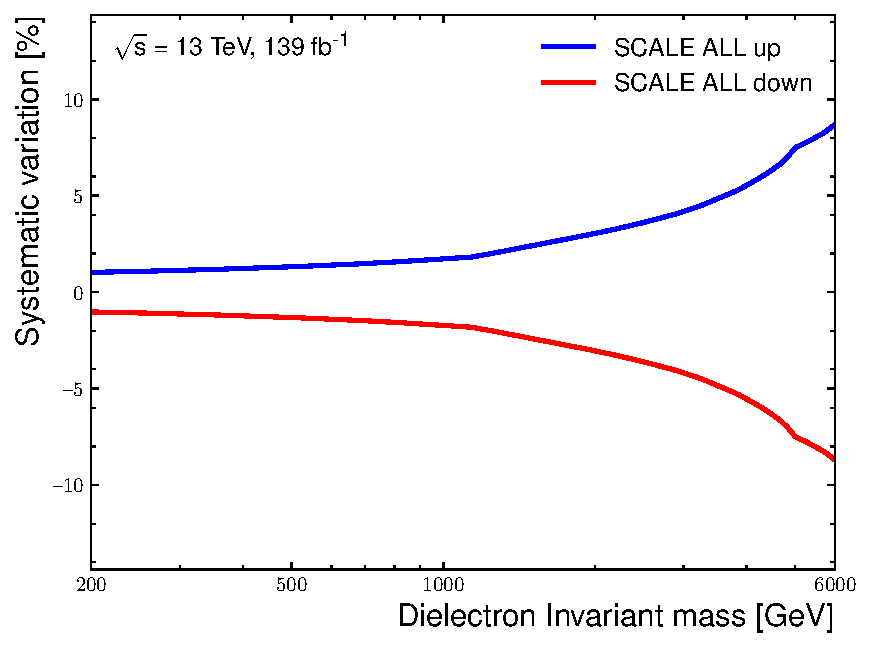
\includegraphics[width=\textwidth]{figures/analysis/datamc/Uncertainties/exp/ee/m_ee_pstOR_EG_SCALE_ALL__1up.pdf}
        \label{fig:uncert:eeScale}
    \end{subfigure}
    \begin{subfigure}[b]{0.42\textwidth}
        \centering
        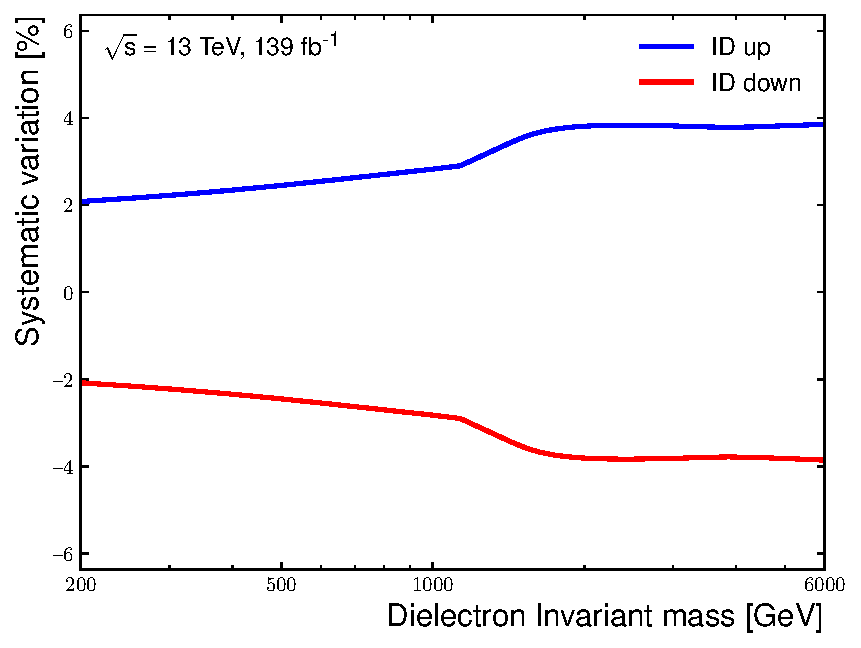
\includegraphics[width=\textwidth]{figures/analysis/datamc/Uncertainties/exp/ee/m_ee_pstOR_EL_EFF_ID_TOTAL_1NPCOR_PLUS_UNCOR__1up.pdf}
        \label{fig:uncert:eeID}
    \end{subfigure}
    \begin{subfigure}[b]{0.42\textwidth}
        \centering
        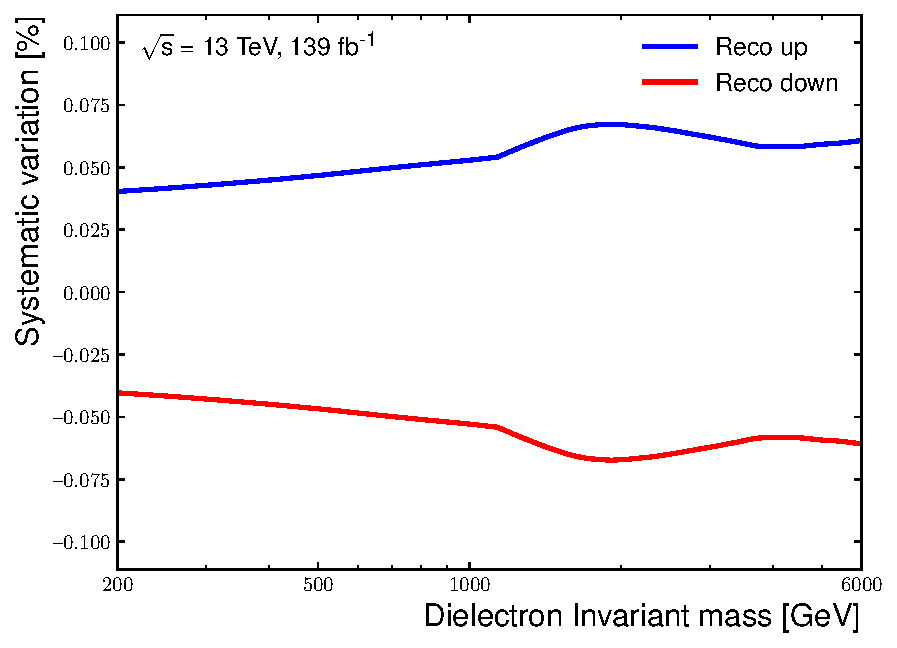
\includegraphics[width=\textwidth]{figures/analysis/datamc/Uncertainties/exp/ee/m_ee_pstOR_EL_EFF_Reco_TOTAL_1NPCOR_PLUS_UNCOR__1up.pdf}
        \label{fig:uncert:eeReco}
    \end{subfigure}
    \begin{subfigure}[b]{0.42\textwidth}
        \centering
        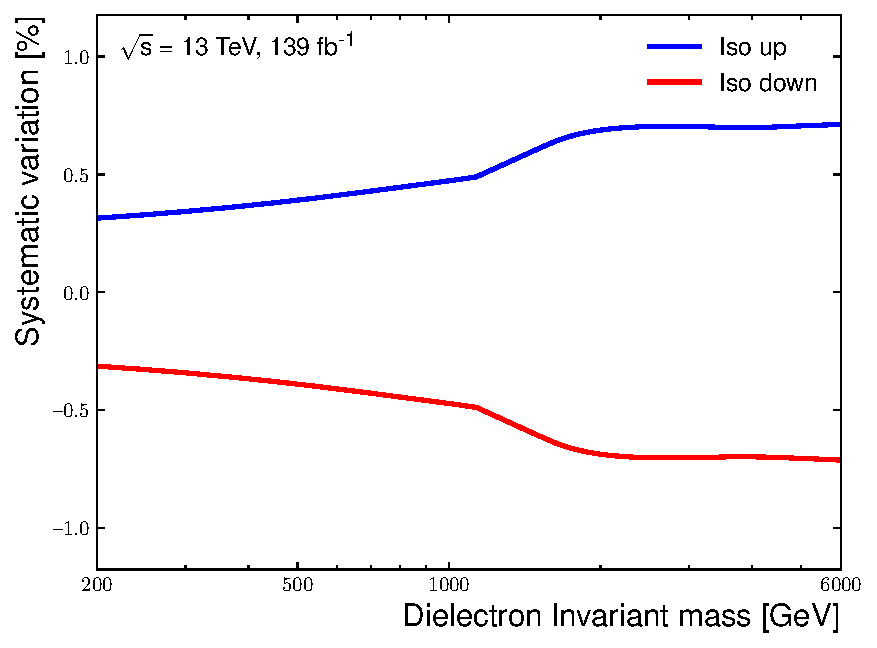
\includegraphics[width=\textwidth]{figures/analysis/datamc/Uncertainties/exp/ee/m_ee_pstOR_EL_EFF_Iso_TOTAL_1NPCOR_PLUS_UNCOR__1up.pdf}
        \label{fig:uncert:eeIso}
    \end{subfigure}
    \begin{subfigure}[b]{0.42\textwidth}
        \centering
        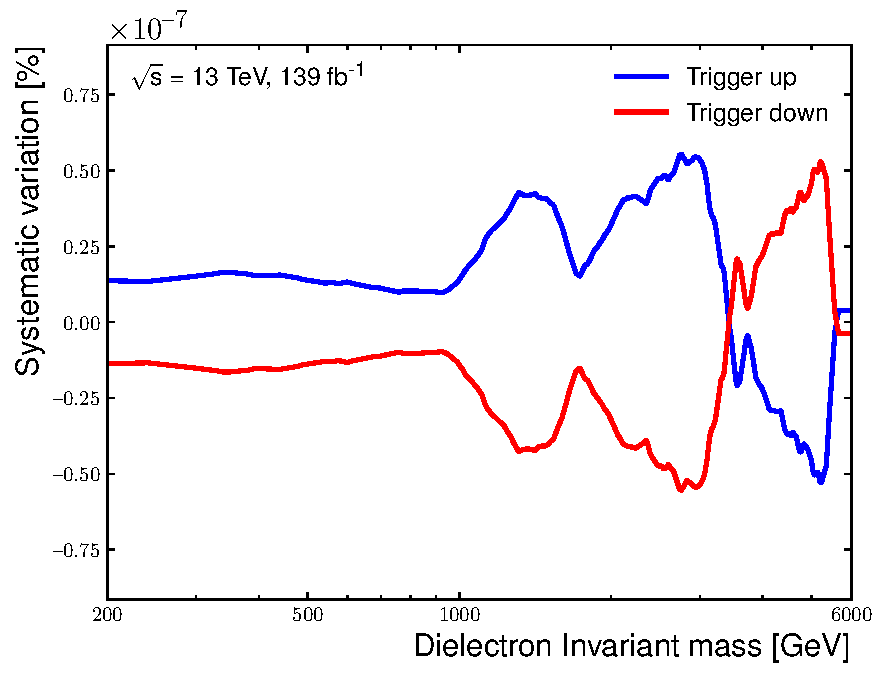
\includegraphics[width=\textwidth]{figures/analysis/datamc/Uncertainties/exp/ee/m_ee_pstOR_EL_EFF_Trigger_TOTAL_1NPCOR_PLUS_UNCOR__1up.pdf}
        \label{fig:uncert:eeTrig}
    \end{subfigure}
    \caption[Electron systematic uncertainties due to experimental sources]{Electron systematic uncertainties due to experimental sources. Shown from left to right and top to bottom, the uncertainty related to electron energy resolution, energy scale, identification, reconstruction, isolation and Trigger.}
    \label{fig:uncert:eeExp}
\end{figure}

\section{Theoretical uncertainties}\label{sec:sysmc:theory}
The theoretical uncertainties considered are only applied to the background modelling simulation samples. High energy searches like the one described in this thesis probe previously uncharted kinematic regions as their mass predictions extend to \SI{}{\tera\electronvolt} energy scales. Therefore, a detailed modelling of the systematic uncertainties related to the knowledge of the partonic structure structure of the proton is required as the kinematic range being probed extends passed the range where the PDF is calculated from data. Differences between the electron and muon channel can be seen due to resolution effects in the detector. 

\subsection{PDF uncertainties}
The PDF uncertainties have been studied for the leading DY background. Each PDF has a set of independent parameters known as eigenvectors associated with it, which can by varied in orthogonal directions to quantify systematic uncertainties associated with a PDF set. For each eigenvector variation at the 90\% Confidence Level in the CT10NNLO~\cite{ct10} parameterisation and {\textsc{VRAP}}~\cite{vrap}, the DY cross section is calculated at NNLO as a function of $m_{\ell\ell}$. The uncertainty due to the PDF variations is taken as the relative deviation of the cross-sections of the PDF variations and the nominal PDF. For each $m_{\ell\ell}$ bin in a histogram, the asymmetric uncertainty on the cross section is calculated using:
\begin{equation}
    \begin{aligned}
    \Delta \sigma^+ = \sqrt{\sum^n_{i=1}\left(\sigma_i^+ - \sigma_0, \sigma^-_i - \sigma_0,0     \right)}, \\
    \Delta \sigma^- = \sqrt{\sum^n_{i=1}\left(\sigma_0 - \sigma_i^+, \sigma_0 -\sigma^-_i,0  \right)}, \\
    \end{aligned}
\end{equation}
where n is the number of PDF eigenvector, $\sigma_i^+/-$ is the cross-section for the higher and lower values for the corresponding PDF eigenvector, and $\sigma_0$ is the cross-section for the central value for the PDF. A total of seven eigenvector variations are considered in this analysis Using the equation the total asymmetric uncertainty at each invariant mass point can be calculated. The effects of the PDF eigenvector variations is shown on \cref{fig:ucnert:eepdfvar,fig:ucnert:mmpdfvar}.
\begin{figure}[h!]
    \centering
    \begin{subfigure}[b]{0.42\textwidth}
        \centering
        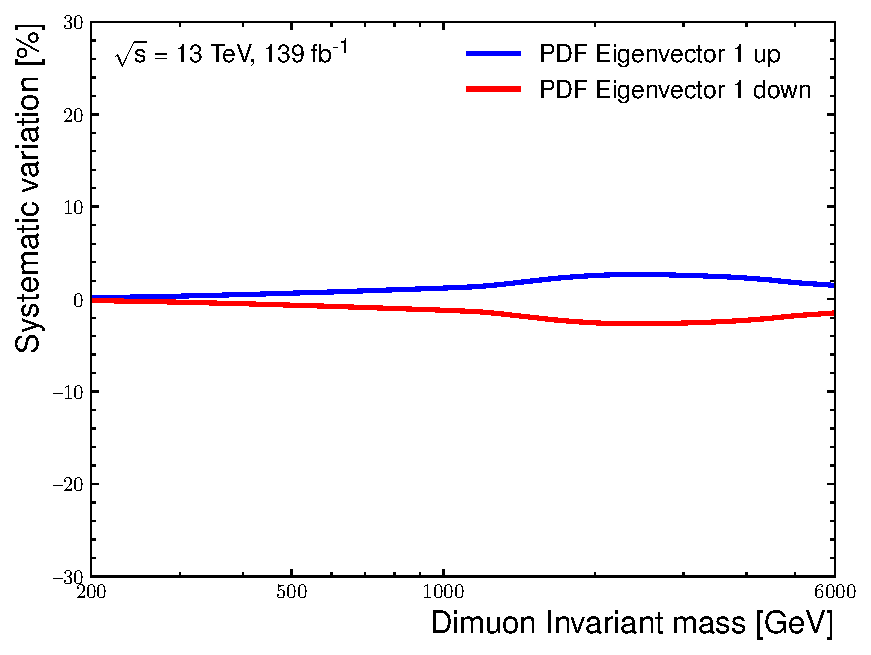
\includegraphics[width=\textwidth]{figures/analysis/datamc/Uncertainties/theory/mm/backgroundTemplate_KF_PDF_EV1.pdf}
        \label{fig:uncert:mmpdfvar1}
    \end{subfigure}
    \begin{subfigure}[b]{0.42\textwidth}
        \centering
        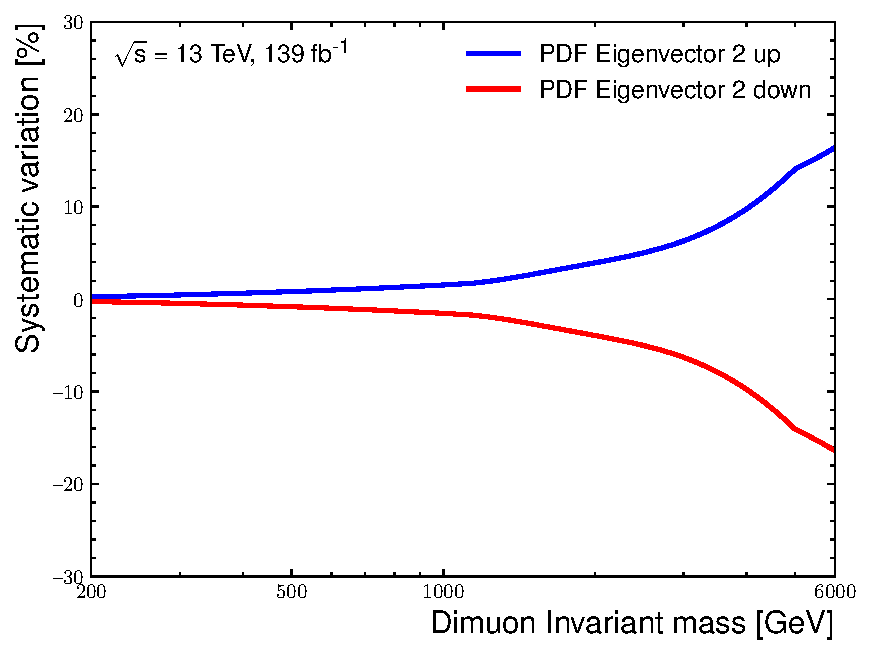
\includegraphics[width=\textwidth]{figures/analysis/datamc/Uncertainties/theory/mm/backgroundTemplate_KF_PDF_EV2.pdf}
        \label{fig:uncert:mmpdfvar2}
    \end{subfigure}
    \begin{subfigure}[b]{0.42\textwidth}
        \centering
        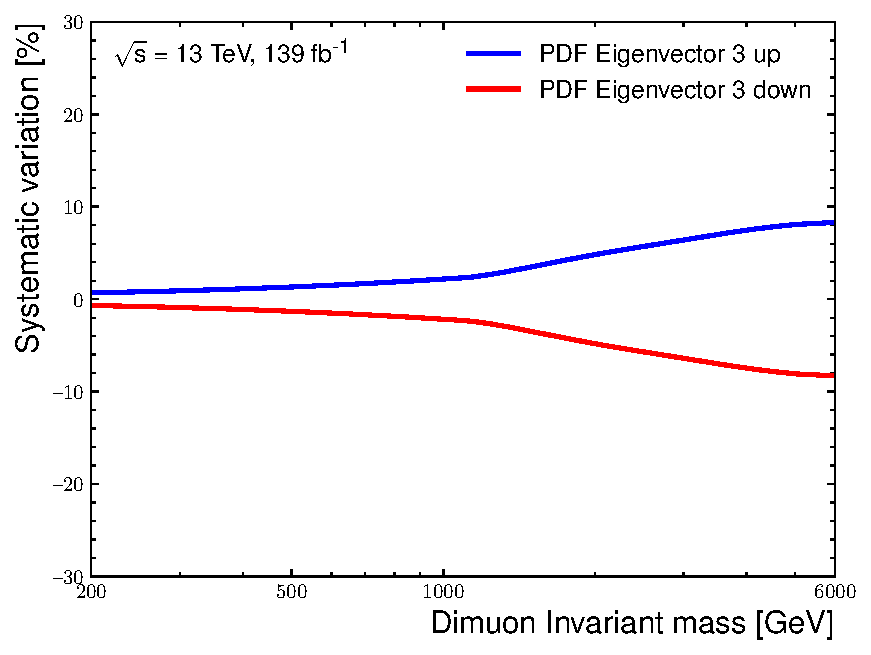
\includegraphics[width=\textwidth]{figures/analysis/datamc/Uncertainties/theory/mm/backgroundTemplate_KF_PDF_EV3.pdf}
        \label{fig:uncert:mmpdfvar3}
    \end{subfigure}
    \begin{subfigure}[b]{0.42\textwidth}
        \centering
        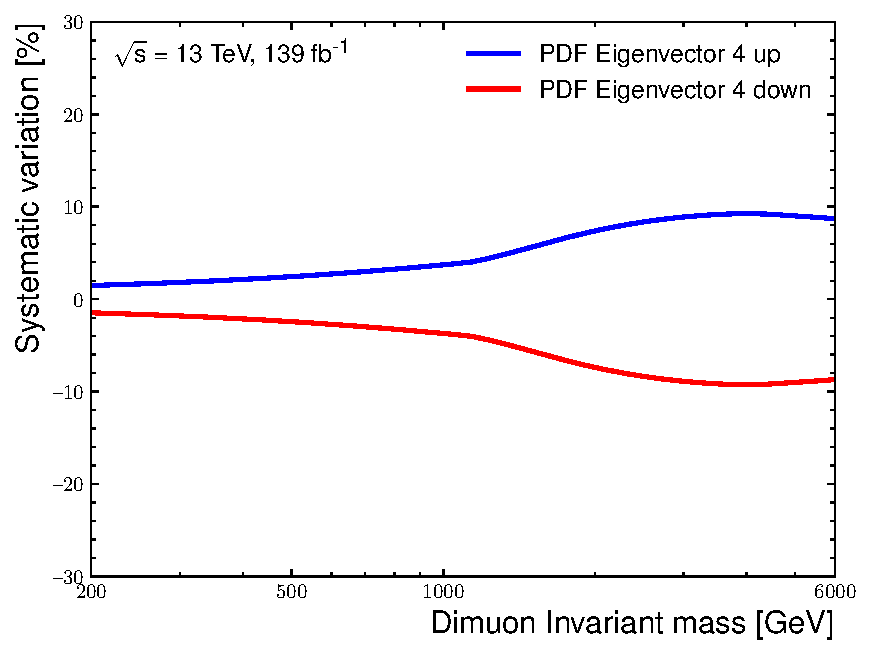
\includegraphics[width=\textwidth]{figures/analysis/datamc/Uncertainties/theory/mm/backgroundTemplate_KF_PDF_EV4.pdf}
        \label{fig:uncert:mmpdfvar4}
    \end{subfigure}
    \begin{subfigure}[b]{0.42\textwidth}
        \centering
        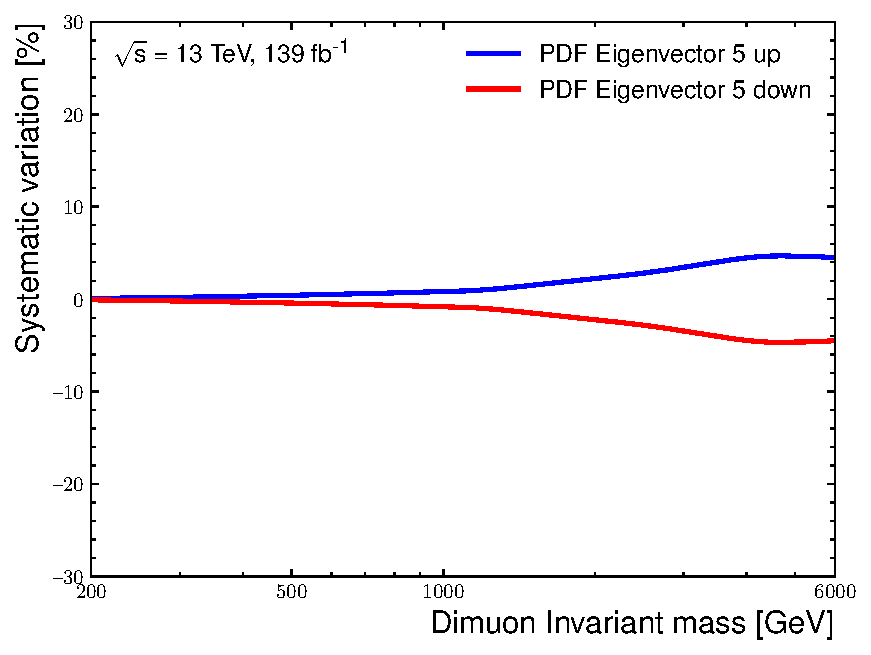
\includegraphics[width=\textwidth]{figures/analysis/datamc/Uncertainties/theory/mm/backgroundTemplate_KF_PDF_EV5.pdf}
        \label{fig:uncert:mmpdfvar5}
    \end{subfigure}
    \begin{subfigure}[b]{0.42\textwidth}
        \centering
        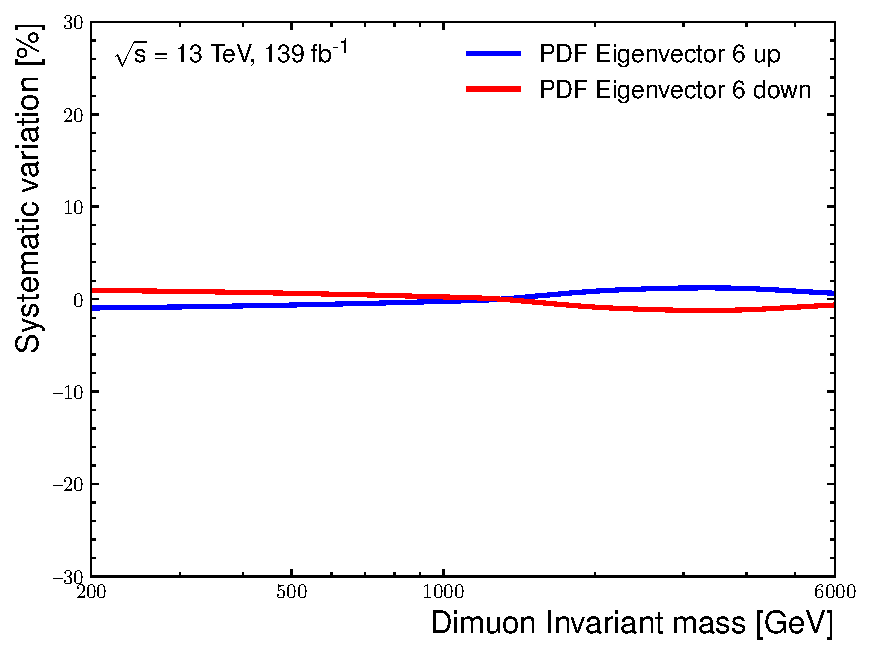
\includegraphics[width=\textwidth]{figures/analysis/datamc/Uncertainties/theory/mm/backgroundTemplate_KF_PDF_EV6.pdf}
        \label{fig:uncert:mmpdfvar6}
    \end{subfigure}
    \begin{subfigure}[b]{0.42\textwidth}
        \centering
        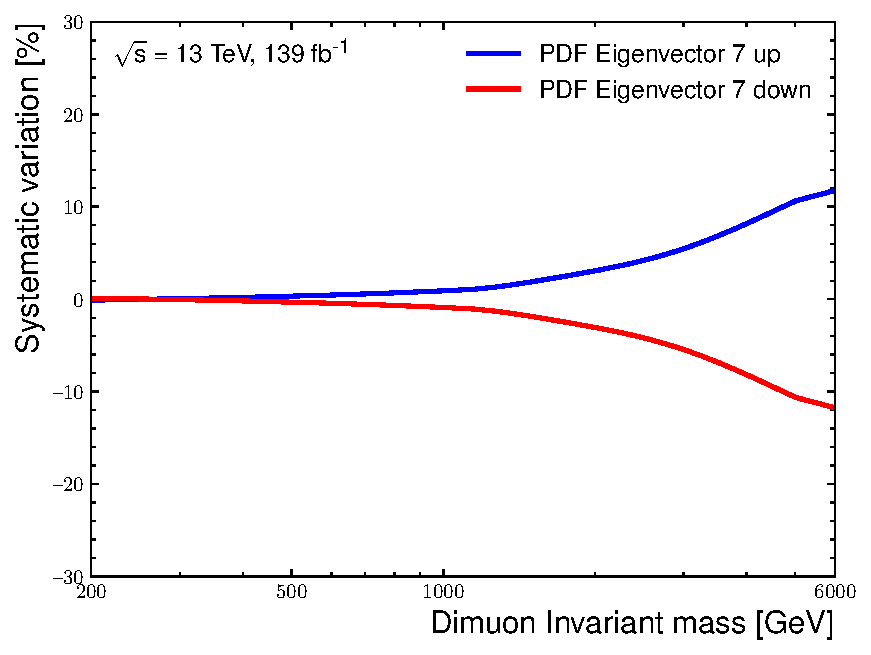
\includegraphics[width=\textwidth]{figures/analysis/datamc/Uncertainties/theory/mm/backgroundTemplate_KF_PDF_EV7.pdf}
        \label{fig:uncert:mmpdfvar7}
    \end{subfigure}
    \caption{Systematic uncertainties due to theoretical sources in the muon channel. Shown from left to right and top to bottom, the uncertainties corresponding to the seven eigenvector variations of the CT10NNLO PDF.}
    \label{fig:ucnert:mmpdfvar}
\end{figure}

\begin{figure}[h!]
    \centering
    \begin{subfigure}[b]{0.42\textwidth}
        \centering
        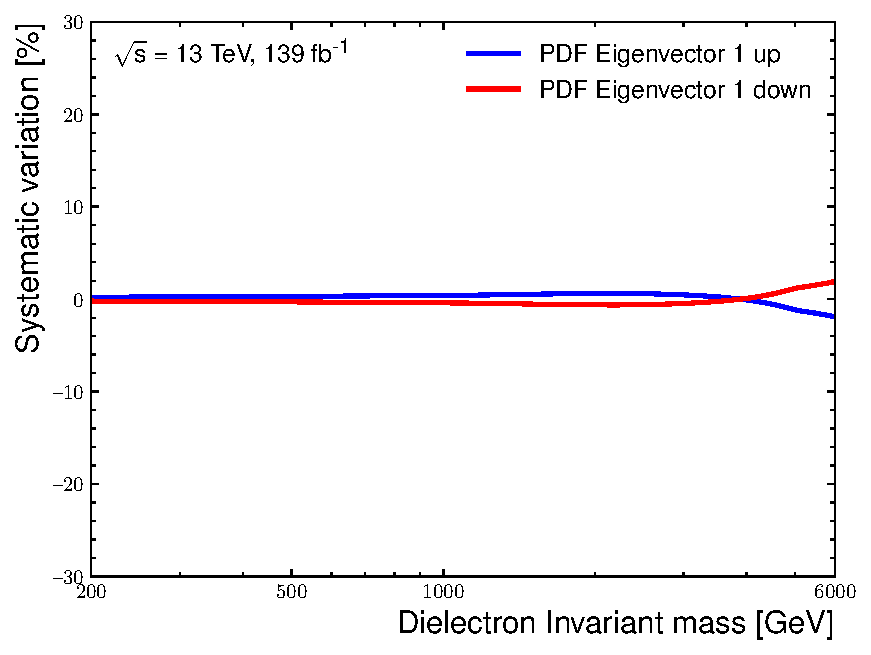
\includegraphics[width=\textwidth]{figures/analysis/datamc/Uncertainties/theory/ee/backgroundTemplate_KF_PDF_EV1.pdf}
        \label{fig:uncert:eepdfvar1}
    \end{subfigure}
    \begin{subfigure}[b]{0.42\textwidth}
        \centering
        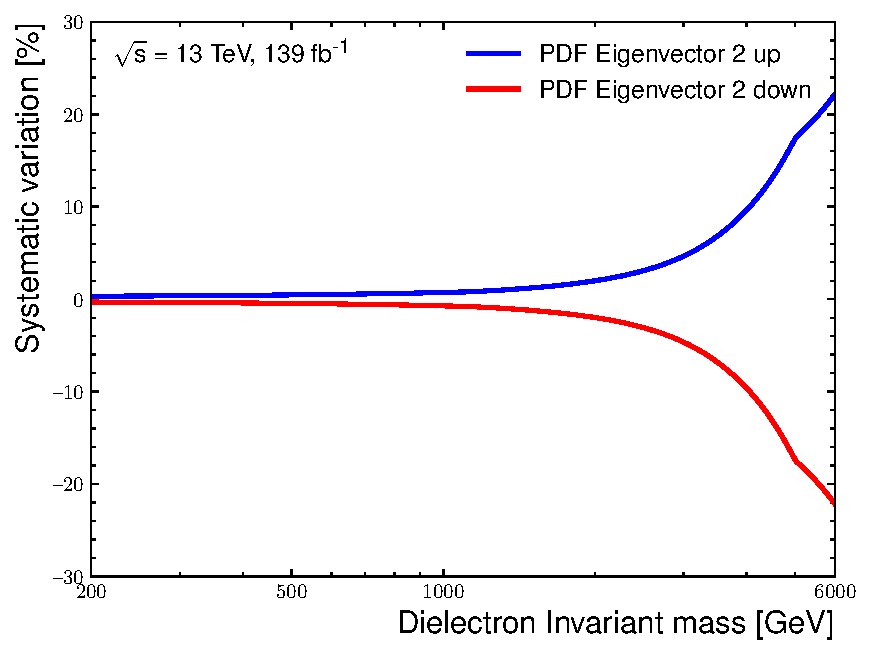
\includegraphics[width=\textwidth]{figures/analysis/datamc/Uncertainties/theory/ee/backgroundTemplate_KF_PDF_EV2.pdf}
        \label{fig:uncert:eepdfvar2}
    \end{subfigure}
    \begin{subfigure}[b]{0.42\textwidth}
        \centering
        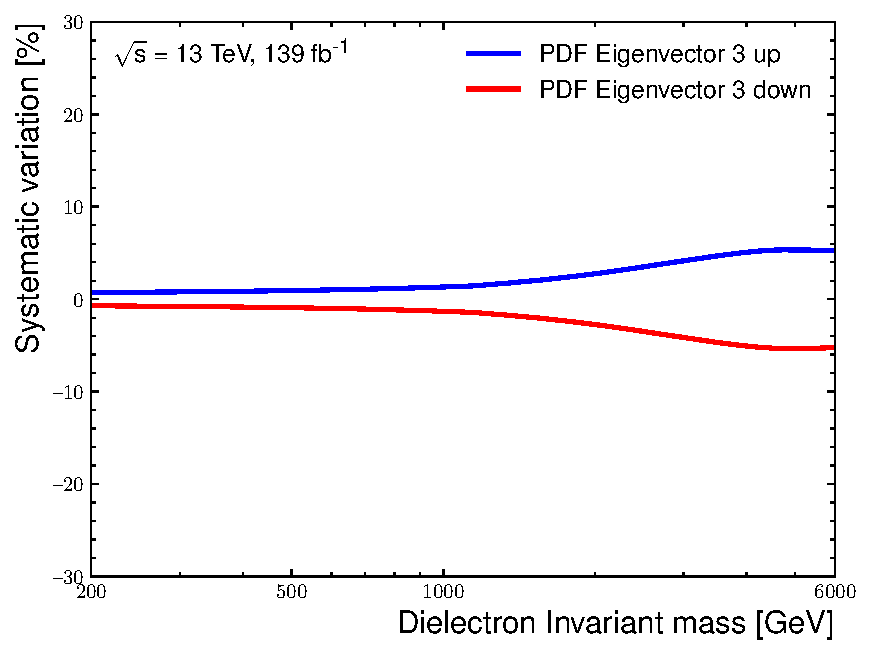
\includegraphics[width=\textwidth]{figures/analysis/datamc/Uncertainties/theory/ee/backgroundTemplate_KF_PDF_EV3.pdf}
        \label{fig:uncert:eepdfvar3}
    \end{subfigure}
    \begin{subfigure}[b]{0.42\textwidth}
        \centering
        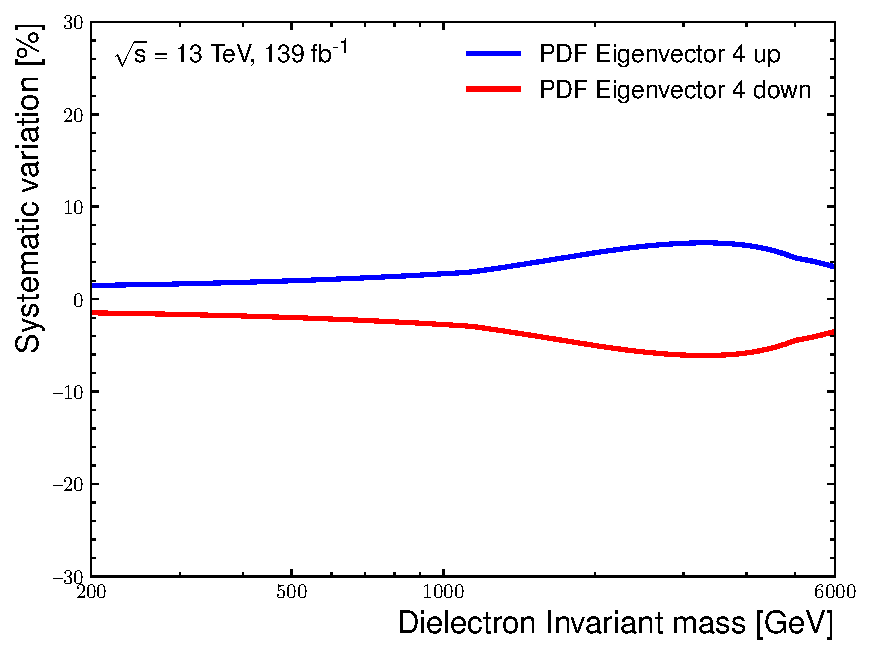
\includegraphics[width=\textwidth]{figures/analysis/datamc/Uncertainties/theory/ee/backgroundTemplate_KF_PDF_EV4.pdf}
        \label{fig:uncert:eepdfvar4}
    \end{subfigure}
    \begin{subfigure}[b]{0.42\textwidth}
        \centering
        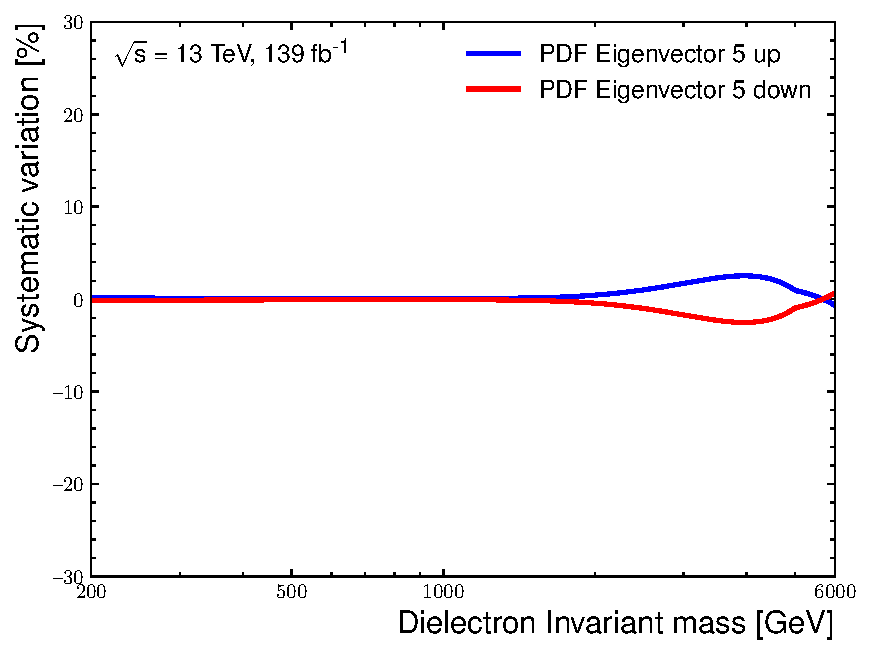
\includegraphics[width=\textwidth]{figures/analysis/datamc/Uncertainties/theory/ee/backgroundTemplate_KF_PDF_EV5.pdf}
        \label{fig:uncert:eepdfvar5}
    \end{subfigure}
    \begin{subfigure}[b]{0.42\textwidth}
        \centering
        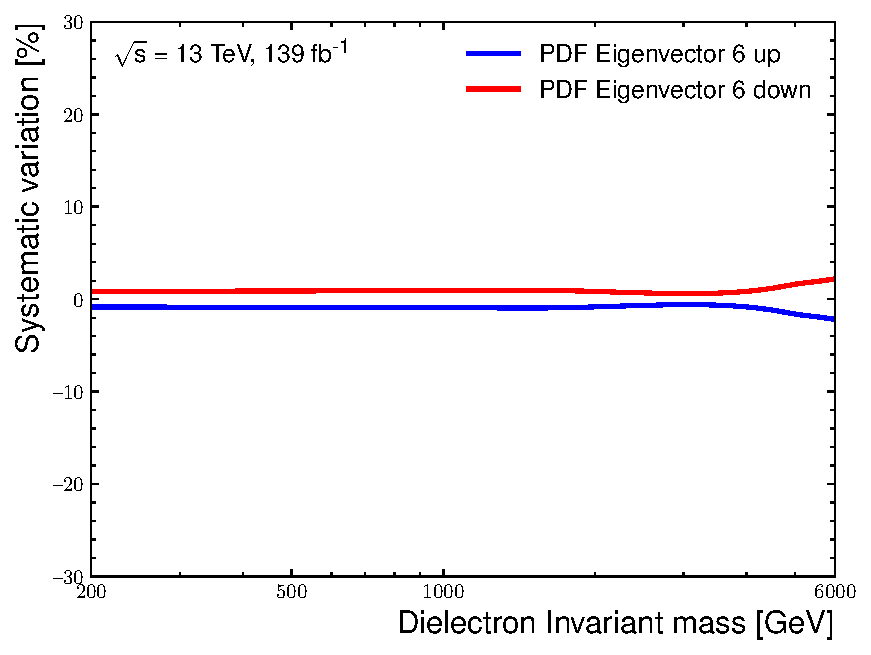
\includegraphics[width=\textwidth]{figures/analysis/datamc/Uncertainties/theory/ee/backgroundTemplate_KF_PDF_EV6.pdf}
        \label{fig:uncert:eepdfvar6}
    \end{subfigure}
    \begin{subfigure}[b]{0.42\textwidth}
        \centering
        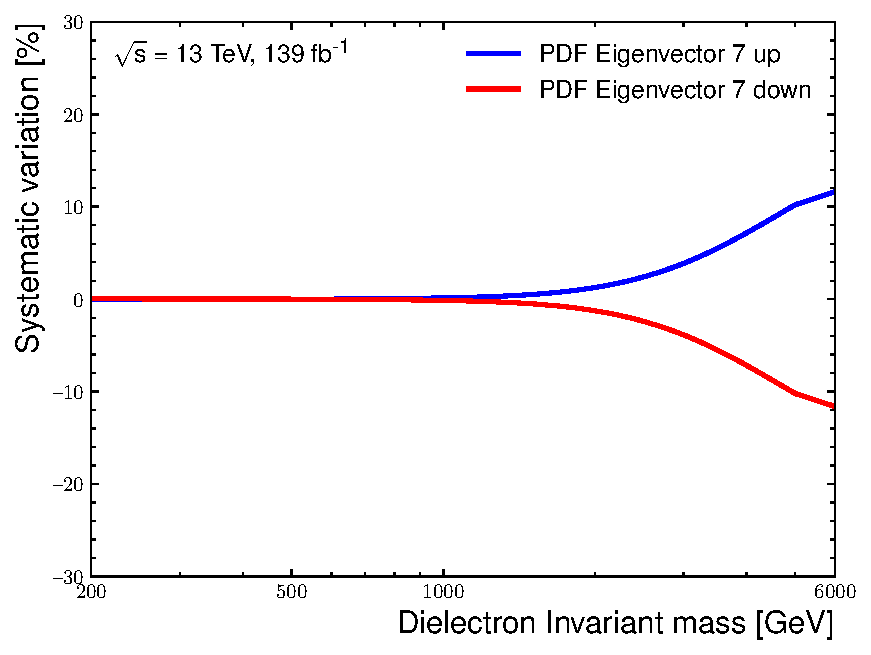
\includegraphics[width=\textwidth]{figures/analysis/datamc/Uncertainties/theory/ee/backgroundTemplate_KF_PDF_EV7.pdf}
        \label{fig:uncert:eepdfvar7}
    \end{subfigure}
    \caption{Systematic uncertainties due to theoretical sources in the electron channel. Shown from left to right and top to bottom, the uncertainties corresponding to the seven eigenvector variations of the CT10NNLO PDF.}
    \label{fig:ucnert:eepdfvar}
\end{figure}

The uncertainty related to the choice of PDF is determined by comparing the central value of CT10NNLO PDF to similar PDFs. Two alternatives for the nominal PDF are considered, the NNPDF3.0 and MMHT14 PDFs. At low masses $< \SI{3}{\tera\electronvolt}$ the PDF sets are in good agreement. At higher masses the PDFs begin to diverge, with some PDF enveloped becoming very large. When the PDF difference between the nominal PDF and an alternative is larger than the uncertainty related to the PDF eigenvector variations, the maximum deviation of the envelope of the comparisons is taken as the PDF choice uncertainty. \cref{fig:uncert:pdfchoice} depicts the PDF choice uncertainty comparing the nominal PDF to NNPDF30 and HERAPDF20 in the electron and muon channels. 
\begin{figure}[h!]
    \centering
    \begin{subfigure}[b]{0.42\textwidth}
        \centering
        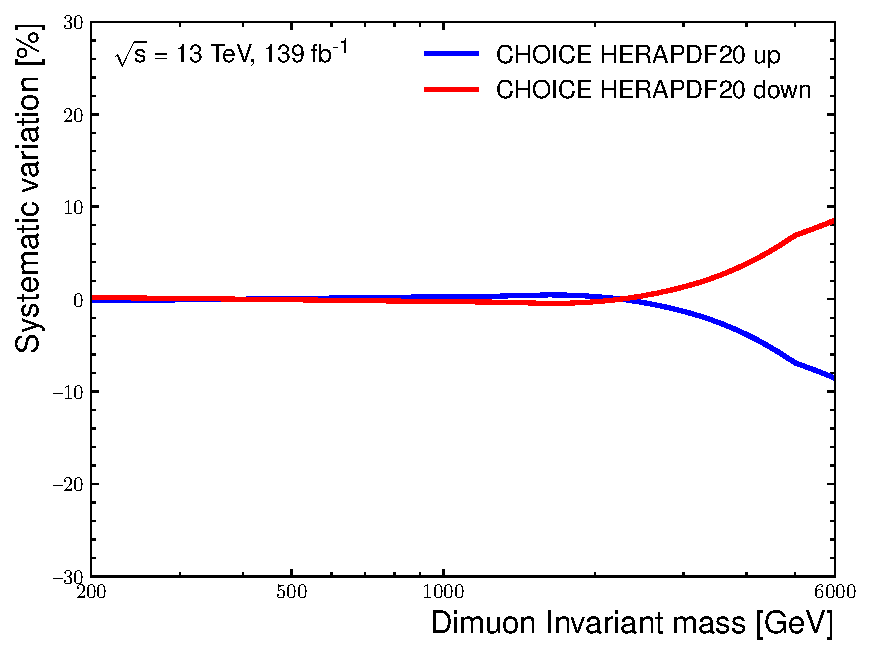
\includegraphics[width=\textwidth]{figures/analysis/datamc/Uncertainties/theory/mm/backgroundTemplate_KF_CHOICE_HERAPDF20.pdf}
        \label{fig:uncert:mmchoiceHERA}
    \end{subfigure}
    \begin{subfigure}[b]{0.42\textwidth}
        \centering
        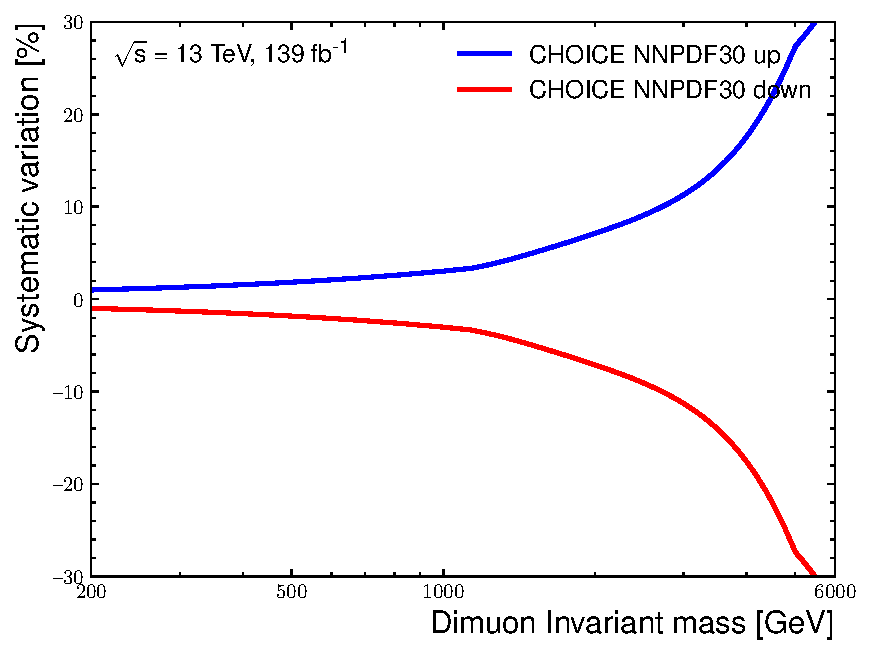
\includegraphics[width=\textwidth]{figures/analysis/datamc/Uncertainties/theory/mm/backgroundTemplate_KF_CHOICE_NNPDF30.pdf}
        \label{fig:uncert:mmchoiceNNPDF}
    \end{subfigure}
    \begin{subfigure}[b]{0.42\textwidth}
        \centering
        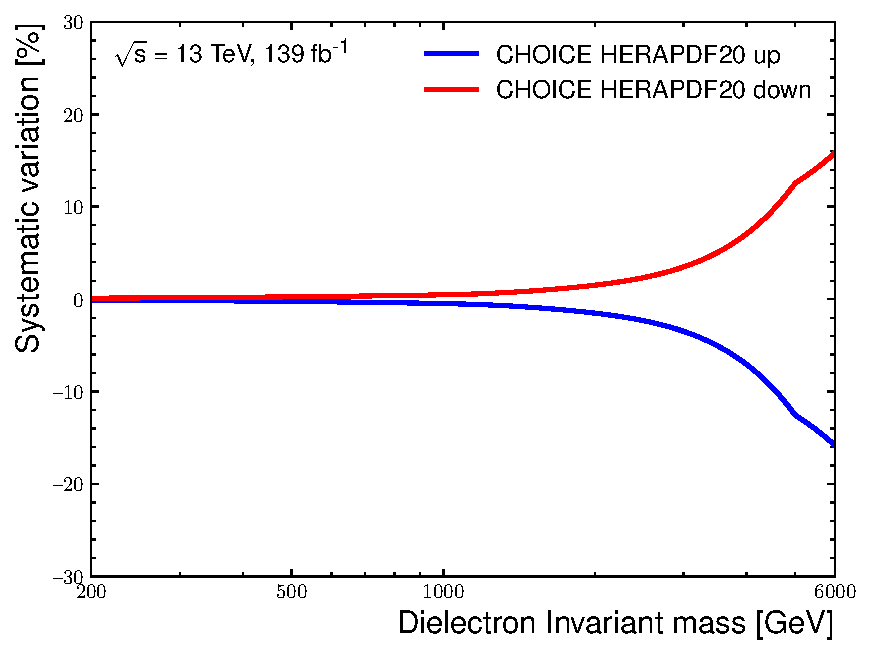
\includegraphics[width=\textwidth]{figures/analysis/datamc/Uncertainties/theory/ee/backgroundTemplate_KF_CHOICE_HERAPDF20.pdf}
        \label{fig:uncert:eechoiceHERA}
    \end{subfigure}
    \begin{subfigure}[b]{0.42\textwidth}
        \centering
        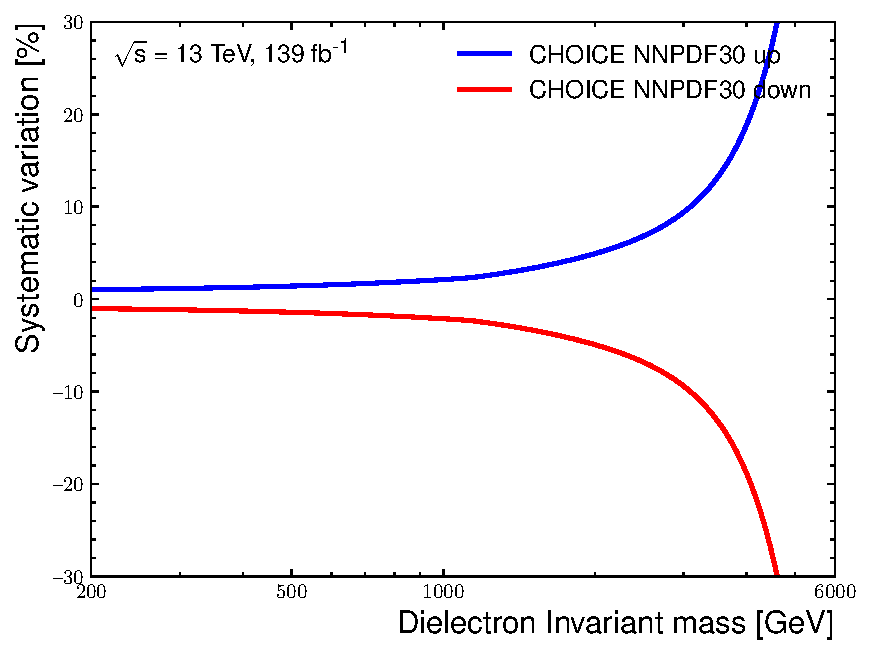
\includegraphics[width=\textwidth]{figures/analysis/datamc/Uncertainties/theory/ee/backgroundTemplate_KF_CHOICE_NNPDF30.pdf}
        \label{fig:uncert:eechoiceNNPDF}
    \end{subfigure}
    \caption{Systematic uncertainties due to the choice of the nominal with respect to HERAPDF20 (left) and NNPDF30 (right) in the muon (top) and electron (right) channels.}
    \label{fig:uncert:pdfchoice}
\end{figure}

The uncertainty on the PDF scales are calculated by varying the factorisation and renormalisation scales of the nominal PDF simultaneously by a factor of two. The resulting maximum variations are taken as the PDF scale uncertainties. \cref{fig:uncert:scales} shows the effects of the scale uncertainty on the invariant mass distribution for the electron and muon channels. 
\begin{figure}[h!]
    \centering
    \begin{subfigure}[h]{0.42\textwidth}
        \centering
        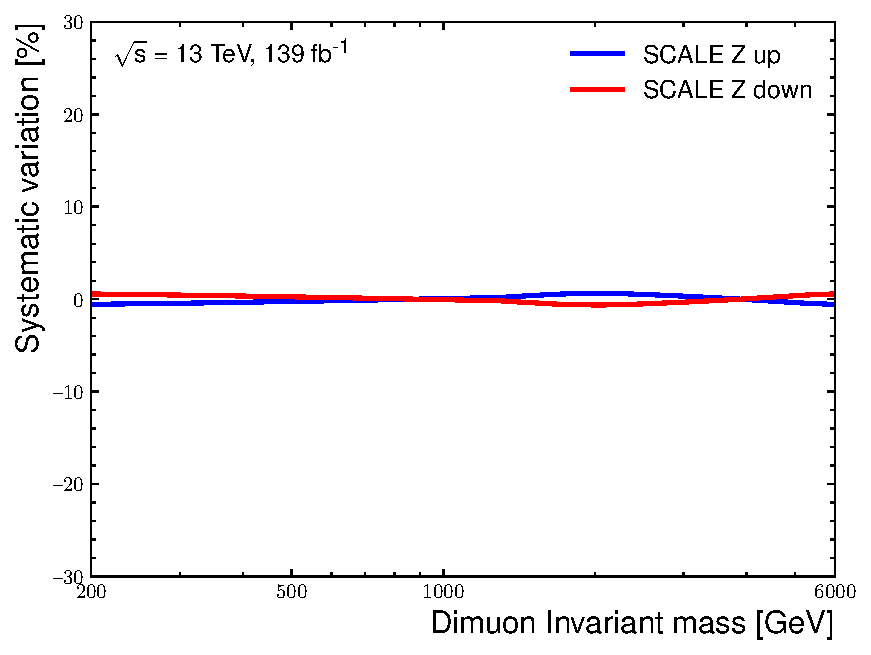
\includegraphics[width=\textwidth]{figures/analysis/datamc/Uncertainties/theory/mm/backgroundTemplate_KF_SCALE_Z__1up.pdf}
        \label{fig:uncert:mmscaleZ}
    \end{subfigure}
    \begin{subfigure}[h]{0.42\textwidth}
        \centering
        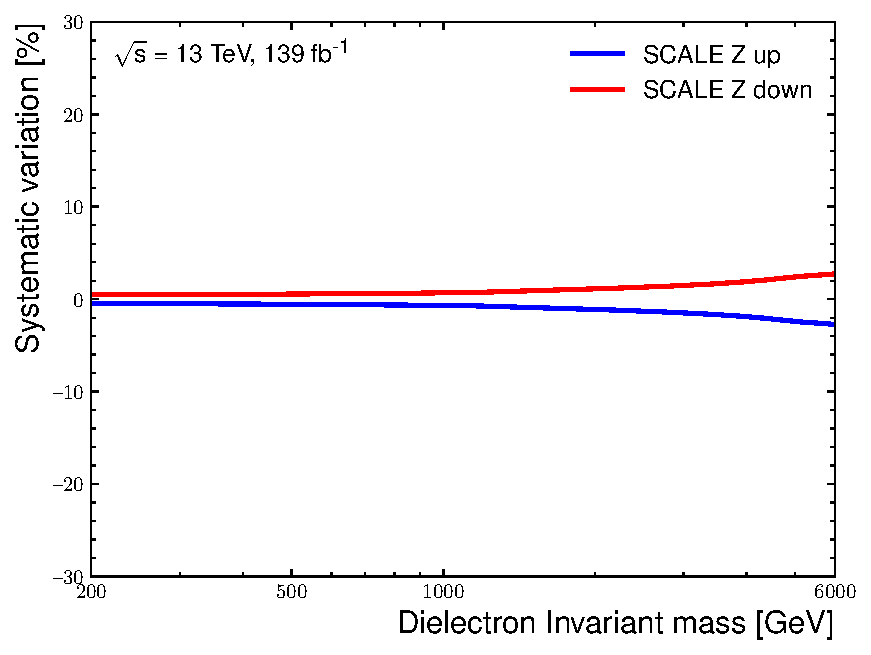
\includegraphics[width=\textwidth]{figures/analysis/datamc/Uncertainties/theory/ee/backgroundTemplate_KF_SCALE_Z__1up.pdf}
        \label{fig:uncert:eescaleZ}
    \end{subfigure}
    \caption{Systematic uncertainties due to factorisation and renormalisation scales of the CT10NNLO PDF in the muon (left) and electron (right) channels.}
    \label{fig:uncert:scales}
\end{figure}

\subsection{Additional theoretical uncertainties}
The uncertainty on the PDF resulting from the uncertainty on the value of the strong coupling constant, $\alpha_s$, is also accounted for in high-mass searches. For the nominal PDF set, the $\alpha_s$ uncertainty is calculated by studying the effect of changing $\alpha_s$ by $\pm 0.003$ from it's nominal value, 0.118 in the cross-section calculation~\cite{Butterworth_2016}.

The combination of EW and QCD corrections is uncertain. Therefore, the EW correction systematic uncertainty was calculated by comparing the additive ($1 + \delta_{EW} + \delta_{QCD}$) versus factored ($(1 + \delta_{EW})(1 + \delta_{QCD})$) computation of the EW \emph{k}-factor. The difference between the two methods is taken as the uncertainty, where the additive computation is used as the nominal in the search. 

\cref{fig:uncert:theoryConstants} show the uncertainties due to the EW and strong coupling constant on the invariant mass distributions for the electron and muon channels. 

\begin{figure}[h!]
    \centering
    \begin{subfigure}[h]{0.42\textwidth}
        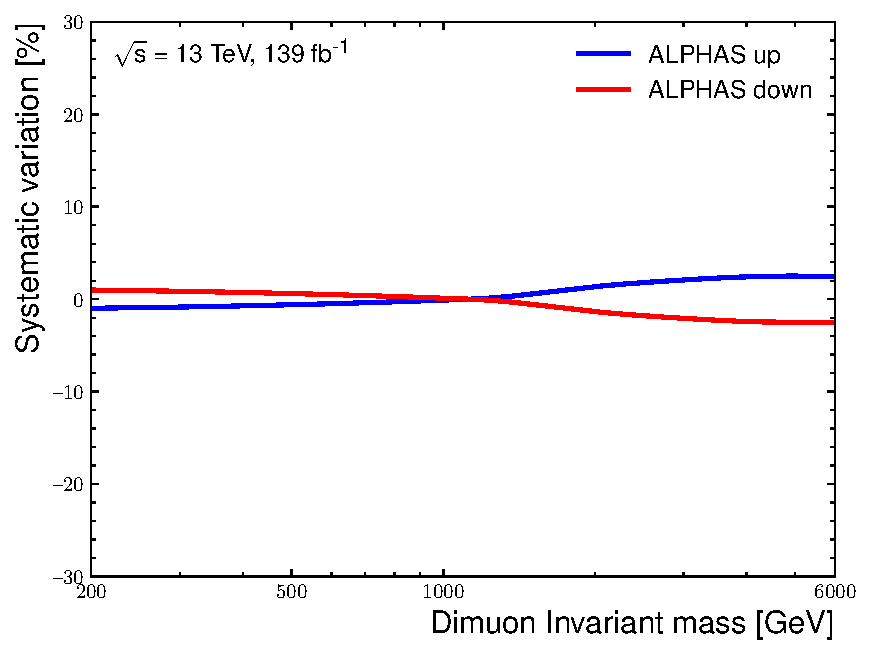
\includegraphics[width=\textwidth]{figures/analysis/datamc/Uncertainties/theory/mm/backgroundTemplate_KF_ALPHAS__1up.pdf}
        \label{fig:uncert:mmalpha}
    \end{subfigure}
    \begin{subfigure}[h]{0.42\textwidth}
        \centering
        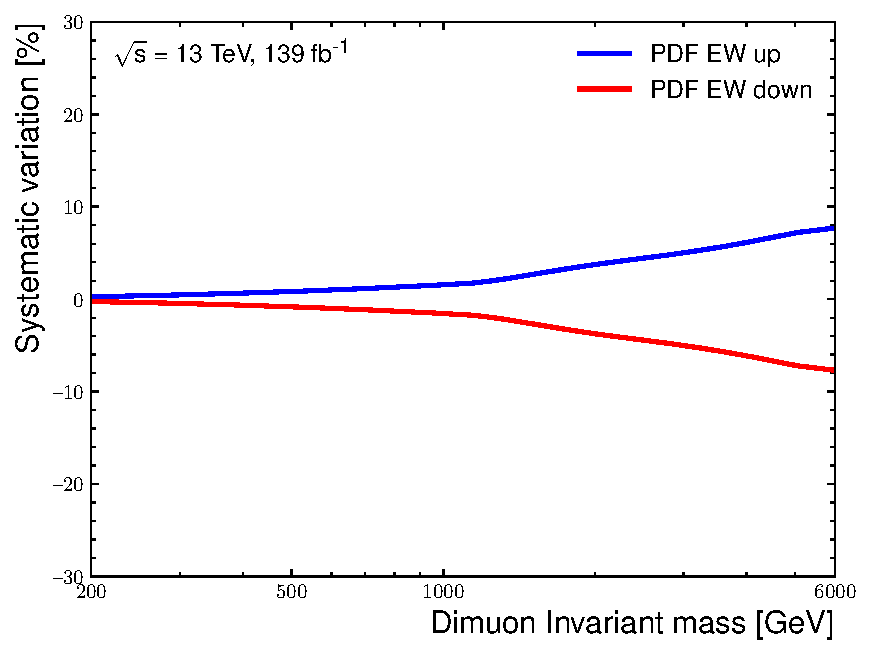
\includegraphics[width=\textwidth]{figures/analysis/datamc/Uncertainties/theory/mm/backgroundTemplate_KF_PDF_EW__1up.pdf}
        \label{fig:uncert:mmEW}
    \end{subfigure}
    \begin{subfigure}[h]{0.42\textwidth}
        \centering
        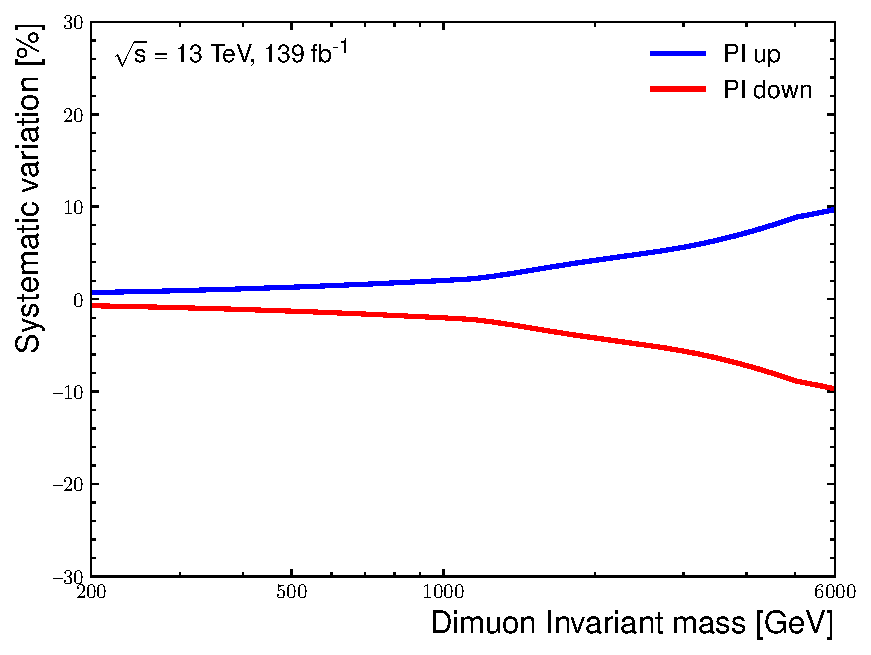
\includegraphics[width=\textwidth]{figures/analysis/datamc/Uncertainties/theory/mm/backgroundTemplate_KF_PI__1up.pdf}
        \label{fig:uncert:mmPI}
    \end{subfigure}
    \begin{subfigure}[h]{0.42\textwidth}
        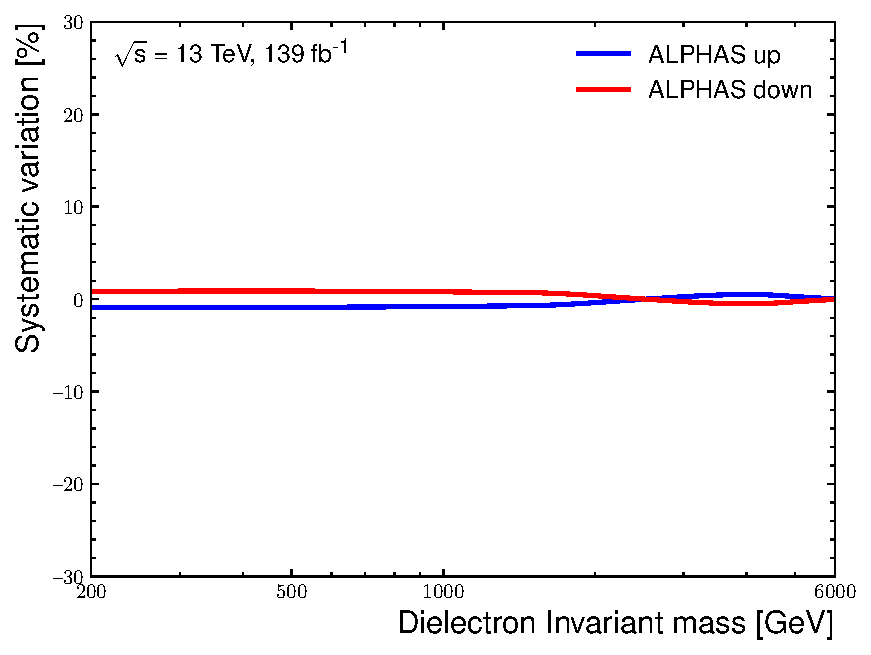
\includegraphics[width=\textwidth]{figures/analysis/datamc/Uncertainties/theory/ee/backgroundTemplate_KF_ALPHAS__1up.pdf}
        \label{fig:uncert:eealpha}
    \end{subfigure}
    \begin{subfigure}[h]{0.42\textwidth}
        \centering
        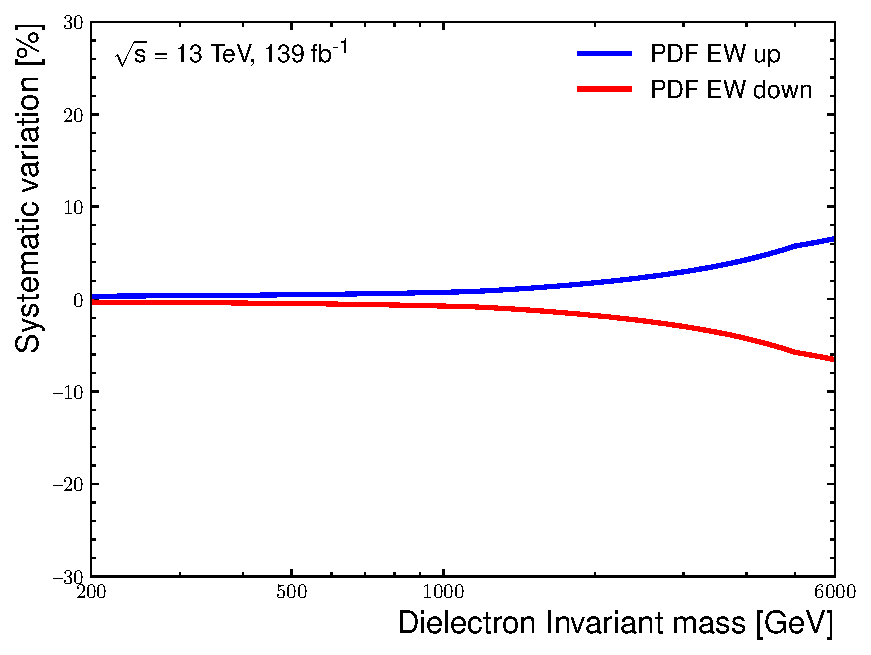
\includegraphics[width=\textwidth]{figures/analysis/datamc/Uncertainties/theory/ee/backgroundTemplate_KF_PDF_EW__1up.pdf}
        \label{fig:uncert:eeEW}
    \end{subfigure}
    \begin{subfigure}[h]{0.42\textwidth}
        \centering
        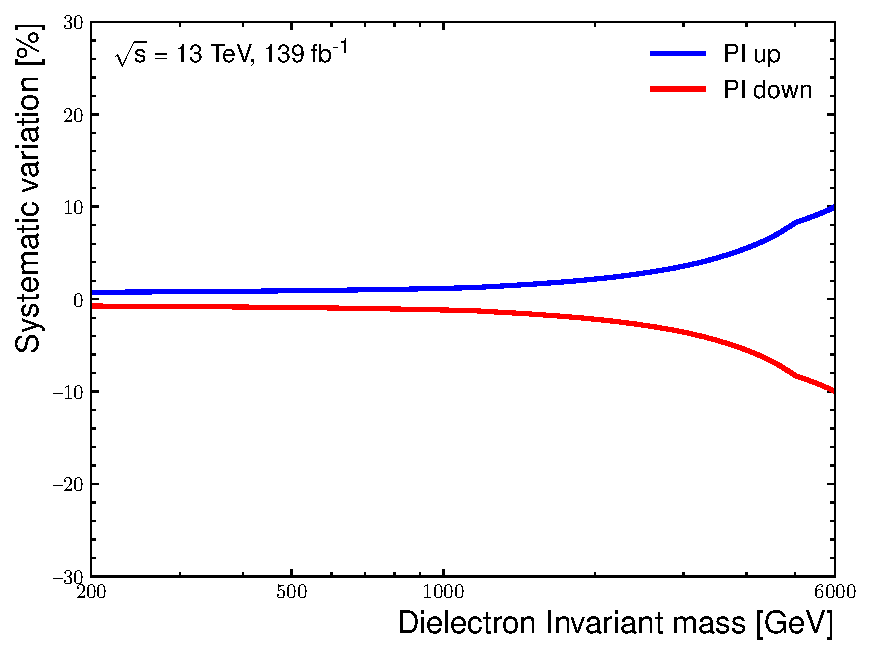
\includegraphics[width=\textwidth]{figures/analysis/datamc/Uncertainties/theory/ee/backgroundTemplate_KF_PI__1up.pdf}
        \label{fig:uncert:eePI}
    \end{subfigure}
    \caption{Systematic uncertainties due to corrections applied to the CT10NNLO PDF. Shown from left to right and top to bottom, the uncertainty related to the strong coupling constant ($\alpha_s$), EW corrections and Photon Induced (PI) corrections in the electron and muon channels.}
    \label{fig:uncert:theoryConstants}
\end{figure}

\clearpage